%!TeX root=../pridetop.tex
\chapter[Chapter \thechapter]{}
	
	
\begin{figure}[t!]
\centering
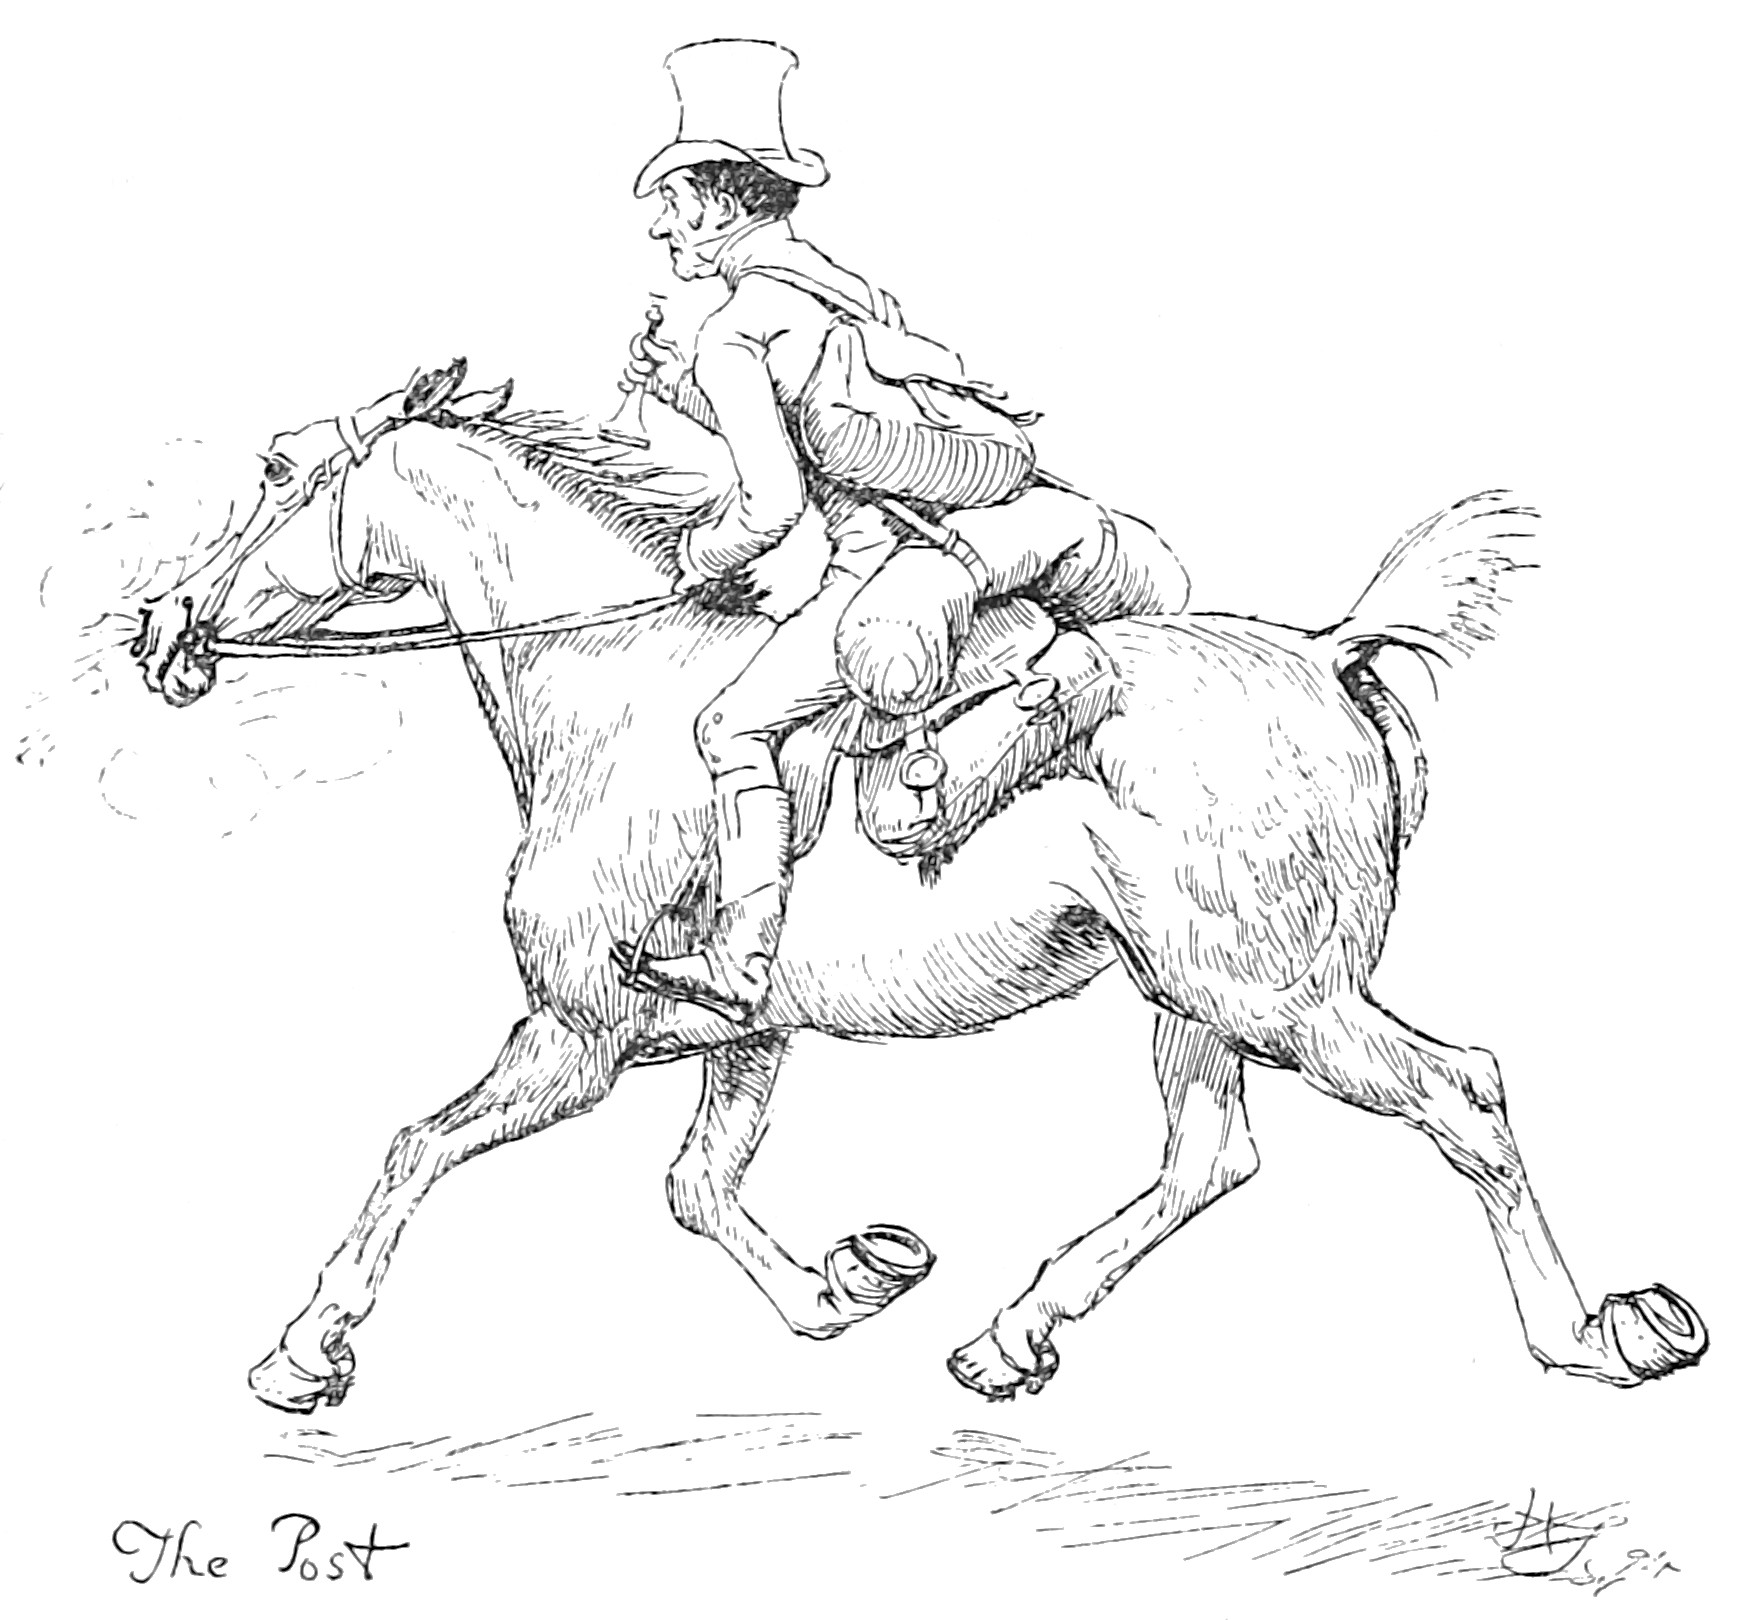
\includegraphics[width=.8\linewidth]{48top}
\captionlistentry{The Post}
\end{figure}


\lettrine[lines=6,image=true]{initials/chap48t}{he}  whole party were in hopes of a letter from Mr Bennet the next morning, but the post came in without bringing a single line from him. His family knew him to be, on all common occasions, a most negligent and dilatory correspondent; but at such a time they had hoped for exertion. They were forced to conclude, that he had no pleasing intelligence to send; but even of \textit{that} they would have been glad to be certain. Mr Gardiner had waited only for the letters before he set off.

When he was gone, they were certain at least of receiving constant information of what was going on; and their uncle promised, at parting, to prevail on Mr Bennet to return to Longbourn as soon as he could, to the great consolation of his sister, who considered it as the only security for her husband's not being killed in a duel.

Mrs Gardiner and the children were to remain in Hertfordshire a few days longer, as the former thought her presence might be serviceable to her nieces. She shared in their attendance on Mrs Bennet, and was a great comfort to them in their hours of freedom. Their other aunt also visited them frequently, and always, as she said, with the design of cheering and heartening them up—though, as she never came without reporting some fresh instance of Wickham's extravagance or irregularity, she seldom went away without leaving them more dispirited than she found them.

All Meryton seemed striving to blacken the man who, but three months before, had been almost an angel of light. He was declared to be in debt to every tradesman in the place, and his intrigues, all honoured with the title of seduction, had been extended into every tradesman's family. Everybody declared that he was the wickedest young man in the world; and everybody began to find out that they had always distrusted the appearance of his goodness. Elizabeth, though she did not credit above half of what was said, believed enough to make her former assurance of her sister's ruin still more certain; and even Jane, who believed still less of it, became almost hopeless, more especially as the time was now come, when, if they had gone to Scotland, which she had never before entirely despaired of, they must in all probability have gained some news of them.

Mr Gardiner left Longbourn on Sunday; on Tuesday, his wife received a letter from him: it told them, that on his arrival he had immediately found out his brother, and persuaded him to come to Gracechurch Street. That Mr Bennet had been to Epsom and Clapham, before his arrival, but without gaining any satisfactory information; and that he was now determined to inquire at all the principal hotels in town, as Mr Bennet thought it possible they might have gone to one of them, on their first coming to London, before they procured lodgings. Mr Gardiner himself did not expect any success from this measure; but as his brother was eager in it, he meant to assist him in pursuing it. He added, that Mr Bennet seemed wholly disinclined at present to leave London, and promised to write again very soon. There was also a postscript to this effect:—

\begin{quote}
I have written to Colonel Forster to desire him to find out, if possible, from some of the young man's intimates in the regiment, whether Wickham has any relations or connections who would be likely to know in what part of the town he has now concealed himself. If there were anyone that one could apply to, with a probability of gaining such a clue as that, it might be of essential consequence. At present we have nothing to guide us. Colonel Forster will, I dare say, do everything in his power to satisfy us on this head. But, on second thoughts, perhaps Lizzy could tell us what relations he has now living better than any other person.
\end{quote}

Elizabeth was at no loss to understand from whence this deference for her authority proceeded; but it was not in her power to give any information of so satisfactory a nature as the compliment deserved.

She had never heard of his having had any relations, except a father and mother, both of whom had been dead many years. It was possible, however, that some of his companions in the ——shire might be able to give more information; and though she was not very sanguine in expecting it, the application was a something to look forward to.

Every day at Longbourn was now a day of anxiety; but the most anxious part of each was when the post was expected. The arrival of letters was the first grand object of every morning's impatience. Through letters, whatever of good or bad was to be told would be communicated; and every succeeding day was expected to bring some news of importance.

But before they heard again from Mr Gardiner, a letter arrived for their father, from a different quarter, from Mr Collins; which, as Jane had received directions to open all that came for him in his absence, she accordingly read; and Elizabeth, who knew what curiosities his letters always were, looked over her, and read it likewise. It was as follows:—

\begin{quotation}

\noindent My dear Sir,

\indent I feel myself called upon, by our relationship, and my situation in life, to condole with you on the grievous affliction you are now suffering under, of which we were yesterday informed by a letter from Hertfordshire. Be assured, my dear sir, that Mrs Collins and myself sincerely sympathize with you, and all your respectable family, in your present distress, which must be of the bitterest kind, because proceeding from a cause which no time can remove. No arguments shall be wanting on my part, that can alleviate so severe a misfortune; or that may comfort you, under a circumstance that must be, of all others, most afflicting to a parent's mind. The death of your daughter would have been a blessing in comparison of this. And it is the more to be lamented, because there is reason to suppose, as my dear Charlotte informs me, that this licentiousness of behaviour in your daughter has proceeded from a faulty degree of indulgence; though, at the same time, for the consolation of yourself and Mrs Bennet, I am inclined to think that her own disposition must be naturally bad, or she could not be guilty of such an enormity, at so early an age. Howsoever that may be, you are grievously to be pitied; in which opinion I am not only joined by Mrs Collins, but likewise by Lady Catherine and her daughter, to whom I have related the affair. They agree with me in apprehending that this false step in one daughter will be injurious to the fortunes of all the others: for who, as Lady Catherine herself condescendingly says, will connect themselves with such a family? And this consideration leads me, moreover, to reflect, with augmented satisfaction, on a certain event of last November; for had it been otherwise, I must have been involved in all your sorrow and disgrace. Let me advise you, then, my dear sir, to console yourself as much as possible, to throw off your unworthy child from your affection for ever, and leave her to reap the fruits of her own heinous offence.\\

\begin{flushright}
I am, dear sir, etc., etc.
\end{flushright}
\end{quotation}

\begin{figure}[tbh]
\centering

\includegraphics[width=.8\linewidth]{48affair}
\captionlistentry{»To whom I have related the affair«}
\end{figure}

Mr Gardiner did not write again, till he had received an answer from Colonel Forster; and then he had nothing of a pleasant nature to send. It was not known that Wickham had a single relation with whom he kept up any connection, and it was certain that he had no near one living. His former acquaintance had been numerous; but since he had been in the militia, it did not appear that he was on terms of particular friendship with any of them. There was no one, therefore, who could be pointed out as likely to give any news of him. And in the wretched state of his own finances, there was a very powerful motive for secrecy, in addition to his fear of discovery by Lydia's relations; for it had just transpired that he had left gaming debts behind him to a very considerable amount. Colonel Forster believed that more than a thousand pounds would be necessary to clear his expenses at Brighton. He owed a good deal in the town, but his debts of honour were still more formidable. Mr Gardiner did not attempt to conceal these particulars from the Longbourn family; Jane heard them with horror. »A gamester!« she cried. »This is wholly unexpected; I had not an idea of it.«

Mr Gardiner added, in his letter, that they might expect to see their father at home on the following day, which was Saturday. Rendered spiritless by the ill success of all their endeavours, he had yielded to his brother-in-law's entreaty that he would return to his family and leave it to him to do whatever occasion might suggest to be advisable for continuing their pursuit. When Mrs Bennet was told of this, she did not express so much satisfaction as her children expected, considering what her anxiety for his life had been before.

»What! is he coming home, and without poor Lydia?« she cried. »Sure he will not leave London before he has found them. Who is to fight Wickham, and make him marry her, if he comes away?«

As Mrs Gardiner began to wish to be at home, it was settled that she and her children should go to London at the same time that Mr Bennet came from it. The coach, therefore, took them the first stage of their journey, and brought its master back to Longbourn.

Mrs Gardiner went away in all the perplexity about Elizabeth and her Derbyshire friend, that had attended her from that part of the world. His name had never been voluntarily mentioned before them by her niece; and the kind of half-expectation which Mrs Gardiner had formed, of their being followed by a letter from him, had ended in nothing. Elizabeth had received none since her return, that could come from Pemberley.

The present unhappy state of the family rendered any other excuse for the lowness of her spirits unnecessary; nothing, therefore, could be fairly conjectured from \textit{that},—though Elizabeth, who was by this time tolerably well acquainted with her own feelings, was perfectly aware that, had she known nothing of Darcy, she could have borne the dread of Lydia's infamy somewhat better. It would have spared her, she thought, one sleepless night out of two.

When Mr Bennet arrived, he had all the appearance of his usual philosophic composure. He said as little as he had ever been in the habit of saying; made no mention of the business that had taken him away; and it was some time before his daughters had courage to speak of it.

It was not till the afternoon, when he joined them at tea, that Elizabeth ventured to introduce the subject; and then, on her briefly expressing her sorrow for what he must have endured, he replied, »Say nothing of that. Who should suffer but myself? It has been my own doing, and I ought to feel it.«

»You must not be too severe upon yourself,« replied Elizabeth.

»You may well warn me against such an evil. Human nature is so prone to fall into it! No, Lizzy, let me once in my life feel how much I have been to blame. I am not afraid of being overpowered by the impression. It will pass away soon enough.«

»Do you suppose them to be in London?«

»Yes; where else can they be so well concealed?«

»And Lydia used to want to go to London,« added Kitty.

»She is happy, then,« said her father, drily; »and her residence there will probably be of some duration.«

Then, after a short silence, he continued, »Lizzy, I bear you no ill-will for being justified in your advice to me last May, which, considering the event, shows some greatness of mind.«

They were interrupted by Miss Bennet, who came to fetch her mother's tea.

»This is a parade,« cried he, »which does one good; it gives such an elegance to misfortune! Another day I will do the same; I will sit in my library, in my nightcap and powdering gown, and give as much trouble as I can,—or perhaps I may defer it till Kitty runs away.«

»I am not going to run away, papa,« said Kitty, fretfully. »If \textit{I} should ever go to Brighton, I would behave better than Lydia.«

»\textit{You} go to Brighton! I would not trust you so near it as Eastbourne, for fifty pounds! No, Kitty, I have at least learnt to be cautious, and you will feel the effects of it. No officer is ever to enter my house again, nor even to pass through the village. Balls will be absolutely prohibited, unless you stand up with one of your sisters. And you are never to stir out of doors, till you can prove that you have spent ten minutes of every day in a rational manner.«

Kitty, who took all these threats in a serious light, began to cry.

»Well, well,« said he, »do not make yourself unhappy. If you are a good girl for the next ten years, I will take you to a review at the end of them.«